\chapter{Virtualization}
\section{Introduction}
Before virtualization tooked place, companies used to have varius servers, but
most of the time they were found to be idle. The problem was that due to OSs
failures, they couldn't run flawlessly more than one application at a time. In
particular, OSs couldn't provide:
\begin{itemize}
    \item\emph{Full isolation of configurations and shared components}: for
    example an application requiring version 1.0 of some library, created conflicts
    with another application requiring a different version for the same library;
    \item\emph{Temporal isolation for performance predictability}: it could
    happen that one application used a lot of resources causing performance
    degradation for another application;
    \item\emph{Strong spacial isolation for security and reliability}: if
    some application crashed it might have compromised others;
\end{itemize}
All of this lead to companies needing to have a lot of different servers running,
even if they were massively underutilized and were consuming a lot of power.

Computing virtualization established because it offered a flexible way to
share hardware resources between different operating systems. This came in hand
with both advantages and disadvantages.

\paragraph{Advantages}
\begin{itemize}
    \item\emph{Isolation}: critical applications can run in different and
    easily isolated OSs. Also, different services can run in the same host,
    into different \emph{virtual machines} that could even use different CPU cores;
    \item\emph{Consolidation}: different OSs can run at the same time on the
    same hardware, thus saving resources and minimising costs and energy
    consumption;
    \item\emph{Flexibility and agility}: system administrators have complete control
    over \emph{virtual machines} execution, and they can pause and restart them.
    Moreover, they might migrate one to a different host, or duplicated it to address a
    workload peak. Finally, it's easy to recover from a disaster (e.g. restarting
    a \emph{VM} from a safe snapshot) or spawn a new \emph{virtual machine};
\end{itemize}
\paragraph{Disadvantages}
\begin{itemize}
    \item\emph{Additional overhead}: since each \emph{virtual machine} needs it
    own OS, more hardware resources are required for each by each server;
    \item\emph{Increased difficulty in handling different hardware}: it might
    be difficult for the virtualization manager to grant some application access
    to special components;
\end{itemize}
Virtualization can be used for both server and desktop virtualization, but its
main usage is in server virtualization. In fact, since more OSs can
run on the same physical machine using a configurable amount of resources, it is
no longer necessary for system admins to buy machines with specific physical
characteristics. Instead, they can just buy \emph{COTS} (Common Off The Shelf)
hardware and, on top of which, create different \emph{virtual machines} with their
required specifications. This is convinient because companies can buy tons of
equivalent servers, put them into a datacenter and virtualise their resources.
Also, buying in large volumes often results in a lower individual price.

\subsection{Some definitions}
Before diving into more technical aspects of virtualization, let's give some
definitions.

\begin{definition}[Layering]
    Layering is a common approch to manage system complexity which allows
    to minimise the interactions among subsystems of a complex system. The
    description of those subsystems is also simplified because each of them is
    abstracted through its interface to the others. Finally, layering allows
    to manage each subsystem individually.
\end{definition}\noindent
For example, a computer can be divided into two main layers: hardware and software,
and software can then be divided into kernel, libraries and applications.
Examples of interfaces between software layers are ISA, ABI and API.

\begin{definition}[Virtual machine (VM)]
    A virtual machine is a software emulation of a physical machine that executes
    both OS and applications as if they were being executed on a physical machine.
\end{definition}\noindent
When taking about \emph{virtual machines} we need to distinguish between two actors:
\begin{enumerate}
    \item\emph{Host OS}: it's the OS that is running on the physical machine and
    that is handling virtualization;
    \item\emph{Guest OS}: it's the OS running on a \emph{virtual machine}, and it
    shouldn't be aware of being running in a virtualised environment ;
\end{enumerate}

\begin{definition}[Hypervisor]
    The hypervisor is the software in charge of the virtualization process,
    meaning that it has to virtualise the hardware resources. This is done by:
    \begin{itemize}
        \item Assigning, when possible, a specific set of resources to each
        virtual machine while granting that each of them doesn't get access
        outside its boundaries;
        \item Arbitring access to shared resources that cannot be partitioned;
    \end{itemize}
\end{definition}
\begin{note}
    The \emph{hypervisors} is also often refered to as \emph{Virtual Machine
    Manager} (\emph{VMM}).
\end{note}
\noindent
The \emph{hypervisor} is often implemented as a Linux-based stripped-off OS
(i.e. an OS with minimum functionalities) to make it more efficient
and more easily securable. The \emph{hypervisor} exports a set of
\q{standard} devices to hosted OSs (i.e. the most common pieces of hardware
that are supported from most OSs).

The \emph{hypervisor} must provide \emph{guest OSs} with a \q{virtual hardware}
whose characteristics are specified in a given hardware profile.
Also, the real hardware may be different from the virtualised one because it
depends on the devices that are exposed by the \emph{hypervisor}.

To allow \emph{guest OSs} to run in a virtualised environment, CPU, memory and
I/O need to be virtualised correctly.

\section{CPU virtualization}
\emph{VMMs} assign one or more CPU cores to each \emph{VM} so that they can run
their OSs. The ISA of the virtualised hardware will usually be the same
of the physical one, but it is not mandatory. Basically, if they're different
there will be an emulation process that will translate messagges between them.
However, since the emulation process works by doing a binary translation between
the two different ISAs, it is too slow to be generally convinient.

Going back to \emph{VMMs}, they must satisfy three characteristics:
\begin{itemize}
    \item The exposed execution environment  must be identical to the
    physical one, so that OSs can run unmodified;
    \item They must have complete control over real system resources, so that
    any \emph{guest OS} accesses only those components it has been grant access
    to;
    \item They must run the virtualised systems efficiently;
\end{itemize}

\subsection{Some definitions}
System based on x86 or x64 architectures are usually modeled into a \emph{privileg
ring} structure. In particular, there are four privileg levels with decreasing
privileges as you move away from the center. In fact, \emph{ring 0} is dedicated
to the OS kerner, and \emph{ring 3} to generic applications.

\begin{figure}[h!]
    \centering
    \img{privileged-ring-model.png}{0.4}
    \caption{\emph{Privilege-ring model}}
\end{figure}

\noindent
Virtualization can use \q{ring de-priviledging}, a technique that runs
\emph{guest OSs} in level greater than \emph{ring 0}, so that they have
limited privileges and therefore can't interfere with each other or with the
\emph{VMM}. The possible models are two:
\begin{itemize}
    \item\emph{0/1/3}: the \emph{VMM} runs at \emph{ring 0}, \emph{guest OSs}
    at \emph{ring 1} and applications at \emph{ring 3}. Since, in x86 architetures,
    some privileges with respect to memory accesses are granted to \emph{ring 0-2},
    \emph{guest OSs} might still interfere with the \emph{VMM};
    \item\emph{0/3/3}: the \emph{VMM} runs at \emph{ring 0}, \emph{guest OSs}
    and applications at \emph{ring 3}. This solves the previous problem, but
    \emph{guest OSs} are no longer protected by malicious applications;
\end{itemize}

\begin{definition}[Privileged instruction]
    A privileged instruction is a CPU instruction that needs to be executed in
    a privileged hardware context.
\end{definition}
\begin{definition}[Sensitive instruction]
    A sensitive instruction is a CPU instruction that can leak information about
    the physical state of the processor.
\end{definition}
\begin{note}
    \emph{Sensitive instructions} are, for example, those that can read the
    register in which the currect CPU privileg level is stored.
\end{note}\noindent
To be virtualizable all CPU's \emph{sensitive instructions} must be
\emph{privileged}.

\begin{definition}[Trap]
    A trap is an event that triggers the switch from an unprivileged context to
    a priviliged one.
\end{definition}\noindent
If a \emph{privileged instruction} is called while the CPU isn't running in
kernel mode (the mode associated to \emph{ring 0}), a \emph{trap} is generated.
So, the CPU jumps to the \emph{Hardware Exception Handler Vector} (HEHV) and
executes that \emph{privileged instruction} in kernel mode.

Situations in which a \emph{trap} can occur can be put in one of three buckets:
\begin{enumerate}
    \item\emph{Exceptions}: invoked when an unexpected error or system mulfunction
    occurs (e.g. \emph{privileged instruction} executed in user mode);
    \item\emph{System call}: invoked by applications in user mode (e.g.
    application asking OS for system I/O);
    \item\emph{Hardware interrupts}: invoked by hardware events in any mode
    (e.g. hardware clock timer triggers events);
\end{enumerate}

\paragraph{System call invocation and hardware interrupts}
In traditional OSs, when an application invokes a \emph{system call}, the CPU
will trap to interrupt handler vector in OS, then will switch to kernel mode
and execute some OS instructions.

Similarly, when an \emph{hardware interrupt} verifies, CPU execution will stop
and it will jump to interrupt handler in OS.

\begin{figure}[h!]
    \centering
    \img{trap-handling-traditional-OSs.png}{0.25}
    \caption{\emph{Trap handling} in traditional OSs}
\end{figure}

\noindent
Diving deeper into \emph{trap handling}, when a \emph{trap} is generated,
userland code (i.e. code outside the kernel) generates a \emph{software
interrupt} (e.g. thorugh the instruction \texttt{INT xx}). Hence, the generic
interrupt routine of the OS is started, and it determines where to jump in the
OS code to serve that interrupt. Finally, kernel jumps to the identified code,
serves the interrupst and then returns control back to the caller (i.e.
instruction \texttt{IRET}). All of this requires to load and parse the content
of several memory locations, so it's rather slow.

A more modern way to serve interrupts uses \texttt{SYSENTER} and
\texttt{SYSEXIT} instructions (\texttt{SYSCALL} and \texttt{SYSRETURN} in
x64 systems) to speed up the process. Practically, userland code writes the
address of the targeted kernel routine in a specific register, then
\texttt{SYSENTER} is called, and the kernel jumps to the selected routine
reading the address from the register, without additional accesses to memory.

\paragraph{Going back to virtualization}
Said this, we can go back to virtualization and talk about the three types
of virtualization that exists:
\begin{enumerate}
    \item\emph{Full virtualization}: \emph{guest OSs} can run unmodified;
    \item\emph{Paravirtualization}: \emph{guest OSs} are aware of being run
    in a \emph{virtual machine}, so they need to be modified;
    \item\emph{Hardware assisted virtualization}: the \emph{hypervisor} exploits
    some functionalities provided by modern CPU chips;
\end{enumerate}

\subsection{Trap \& emulate paradigm}
This paradigm allows \emph{full virtualization} and provides that \emph{guest
OSs} run in an unprivileged environment, hence when a \emph{privileged
instruction} has to be executed, a \emph{trap} is launched by the CPU. Then,
that \emph{trap} is intercepted by the \emph{VMM} that emulates the effect of
the \emph{privileged instruction} for the caller (of course, only if it's
legitimate) and, at the end, gives control back to \emph{guest OS}.

Actually, when the \emph{VMM} intercepts a \emph{trap} it behaves differently
based on the event that caused it. If it was causes by an application, then the
\emph{VMM} passes it direcctly to the \emph{guest OS}. On the other hand, if it
was caused by the \emph{guest OS} itself, the \emph{VMM} handles it by
modifying the state of the \emph{virtual machine}.

\paragraph{System call handling}
\mbox{}

\bigskip\noindent
\begin{minipage}[t]{0.48\textwidth}
    When a \emph{system call} happens, CPU traps it to interrupt handler vector
    of the \emph{VMM}. This then jumps back to the \emph{guest OS}. All of this,
    results in extra context switch operations and performance deteriorates
    further if \emph{guest OS} isn't able to handle the interrupt
    routine by itself. So, time spent to execute a single \emph{system call} might
    be 10 times greater than what it would have been required by the \emph{host
    OS}.
\end{minipage}
\begin{minipage}[t]{0.48\textwidth}
    \centering
    \strut\vspace*{-\baselineskip}\newline
    \img{trap-handling-trap-and-emulate1.png}{0.8}
\end{minipage}

\newpage
\paragraph{Privileged instruction handling}
\mbox{}

\bigskip\noindent
\begin{minipage}[t]{0.48\textwidth}
    When a \emph{privileged instruction} is executed it will be trapped to
    \emph{VMM} who will emulate it. After that, \emph{VMM} will give control back
    to the caller.
\end{minipage}\hfill
\begin{minipage}[t]{0.48\textwidth}
    \centering
    \strut\vspace*{-\baselineskip}\newline
    \img{trap-handling-trap-and-emulate2.png}{0.8}
\end{minipage}

\paragraph{Hardware interrupt handling}
\mbox{}

\bigskip\noindent
\begin{minipage}[t]{0.48\textwidth}
    When a \emph{hardware interrupt} is launched, CPU will trap it to interrupt
    handler of \emph{VMM} that then will jump to the corresponding interrupt
    handler of the \emph{guest OS}.
\end{minipage}\hfill
\begin{minipage}[t]{0.48\textwidth}
    \centering
    \strut\vspace*{-\baselineskip}\newline
    \img{trap-handling-trap-and-emulate3.png}{0.8}
\end{minipage}

\paragraph{Problems with systems virtualization}
In this paradigm, each time a \emph{privileged instruction} is executed in an
unprivileged context, a \emph{trap} has to be generated and detected by the
\emph{VMM}. As we've just seen, these actions are time-consuming.

This process isn't necessary for all architetures, but unfortunatly,
it is in x86 and x64 architectures, which are the most common. Moreover, these
architectures present some \emph{sensitive instructions} (e.g. \texttt{POPA},
\texttt{POPF}) that don't trap when executed in an unprivileged context, hence,
these architectures are said to be \q{non-virtualizable}.

\paragraph{Possible solutions}
So, we have some \emph{sensitive instructions} that don't \emph{trap} and,
consequently, the \emph{VMM} cannot emulate their correcct behavior during
execution.

To address this problem, we can change virtualization paradigm, or introduce
some code into the \emph{VMM} that parses the instruction stream to dynamically
detect all \emph{sensitive instructions}. Then, we can both use
interpretation and binary translation. Interpretation is an old and slow approch
in which emulating a single ASM instruction originates an overhead of one order
of magnitude at least. Binary translation, on the other hand, introduces a
lower performance overhead.

\paragraph{Dynamic binary translation}
The idea behind this approch is to dynamically translate \q{non-virtualizable}
ISA to a virtualizable one during run time. In particular, dynamic means that
translation is done on-the-fly at execution time and interleaved with normal
code execution. Binary means that \emph{VMM} translates binary code instead of
source code and this is more efficient.

One pro of this technique is that it still allows \emph{full virtualization}
without needing specific hardware support, but virtualization overhead is still
too high and several instructions or execution patterns (e.g. \emph{system call})
are significantly slower than real execution.

\begin{note}
    We could use caching techniques to recognize significant instruction patterns
    and increase translation speed.
\end{note}
\begin{note}
    Original VMware \emph{VMM} combined \emph{Trap \& emualte} with a system
    level \emph{Dynamic Binary Translation}. \emph{Guest OSs} run at \emph{ring 1}
    and \emph{VMM} inspected code dynamically to swap non-trappable portions of
    code with \q{safe} instructions.
\end{note}

\subsection{Paravirtualization}
The idea that drives this paradigm is to let \emph{guest OSs} know that
they're running in a virtualised environment  and that, in some case, they'll
have to leave control to a \emph{VMM}. So, \emph{guest OSs} are explicitly
modified to be virtualizable, changing the interface provided to make them
easier to implement.

In particular, \emph{system calls} and \q{non-virtualizable instructions} are
replaced with specific \emph{hypervisor calls} (\emph{hypercalls}). Hence,
they won't trap anymore and all the \emph{trap \& emulate} process can be
removed. Of course, modifications don't affect the \emph{ABI}, so applications
can be executed without further changes.

\emph{Guest OSs} are explicitly deprivileged meaning that they know they're being
executed at \emph{ring 1}. This allows to introduce in \emph{guest OS}
kernels efficient mechanisms that ease the communication with the
\emph{hypervisor}:
\begin{itemize}
    \item\emph{Guesto-to-Hypervisor}: \emph{privileged instructions} are replaced
    with synchronous paravirtualised equivalent \emph{hypercalls};
    \item\emph{Hypervistor-to-Guest}: \emph{hypervisor} can notify certain events
    asynchronously to the \emph{guest};
\end{itemize}

\bigskip\noindent
Talking about pros and cons in a paravirtualized environment, only modifiable
OSs can be used, because it's necessary to access their source code.

Performance are surely higher than those of \emph{Trap \& emulate paradigm}
because neither emulation nor translation are required, hence \emph{VMM}
implementation is also simpler and faster.

\subsection{Hardware assisted virtualization}
Up to this point, we still have two unsolved issues: complex implementation of
\emph{VMMs} and necessity to provide full virtualization for most of x86 and x64
systems (most of them weren't still modifiable).

\emph{Hardware assisted virtualization} aims at providing a solution to those
problems by proposing an efficient \emph{Trap \& emulate} approach to
virtualization thanks to an additional hardware support.

This is based on the idea of avoiding \emph{sensitive instructions}, either
because they can be \q{promoted} to \emph{privileged} or because the \emph{VMM}
can dynamically configure which instructions have to be trapped. There are some
instructions then, that cause \emph{virtual machines} to exit unconditionally
(e.g. \texttt{INVD} instruction for CPU internal cache invalidation) and therefore
can never be executed in a virtualised non-root environment. Finally, all
events and some other instructions can be configured to operate conditionally
using \emph{virtual machine} execution control fields.

To do all of this, processors are provided with an additional running mode
named \emph{Virtual Machine eXtensions} (\emph{VMX}). When this mode is enabled,
CPU will activate two different running modes called \emph{operating levels}
that are: \emph{non-root mode} and \emph{root mode}. These modes still works
with the usual \emph{privileg-ring} structure.

\begin{figure}[h!]
    \centering
    \img{hav.png}{0.35}
    \caption{\emph{Hardware assisted virtualization} modes}
\end{figure}\noindent
The \emph{VMM} runs al \emph{ring 0} in \emph{root-mode}, while \emph{guest OSs}
run at \emph{ring 0} in \emph{non-root mode}. Of course applications still run
at \emph{ring 3} in \emph{non-root mode}.

\paragraph{VMX instructions}
If sytem code tries to execute instructions violating isolation of the \emph{VMM}
or that must be emulated via software, hardware \emph{traps} it and switches back
to the \emph{VMM}. CPU enters \emph{non-root mode} via the new \texttt{VMLAUNCH}
and \texttt{VMRESUME} instructions, and it returns to \emph{root mode} for a
number of reasons, collectively called \emph{VM exits}.

\emph{VM exits} should return control to the \emph{VMM}, that should complete
the emulation of the action that the \emph{guest} code was trying to execute, then
give control back to the \emph{guest} by re-entering \emph{non-root mode}. All
the new \emph{virtual machine} instructions are only allowed in \emph{root mode}.

For example, while in \emph{non-root mode}, \texttt{INT xx} instruction may cause
a swich from \emph{non-root user mode} to \emph{non-root kernel mode}, and
\texttt{IRET} may return from \emph{non-root kernel mode} back to \emph{non-root
user mode}.

\bigskip\noindent
So, when a trapping condition is triggered, \emph{VMM} takes control of the
execution and emulates the correct behaviour. Transition between \emph{root}
and \emph{non-root mode} is realized through:
\begin{itemize}
    \item\emph{VM entry}: from \emph{VMM} to \emph{guest};
    \item\emph{VM exit}: from \emph{guest} to \emph{VMM};
\end{itemize}\noindent
When this happens, registers and address spaces are swapped in a single atomic
operation and, as we would expect, this remains the main source of overhead.

\paragraph{Virtual machine control structure}
To mantain \emph{virtual machines} state and control information \emph{VMM}
uses a particular structure called \emph{Virtual Machine Control Structure}
(\emph{VMCS} or \emph{VMCB}). It concretely represents the control panel of
the \emph{virtual machine}, storing information about \emph{guest} state,
\emph{host} processor and control data (e.g. trapping condition). It also
mirrors all register modifications needed to set a certain configuration in
\emph{guest OSs}. \emph{VMCS} introduced dedicated instructions to modify it:
\texttt{VMWRITE} and \texttt{VMREAD}.

\begin{figure}[h!]
    \centering
    \img{vmcs.png}{0.4}
    \caption{\emph{Virtual Machine Control Structure}}
\end{figure}

\section{Memory virtualization}
\subsection{Memory management in general}
Modern operating systems use a \emph{memory paging} technique to access, as
contiguous, dispersed locations in the physical memory. In particular, the main
memory (RAM) is divided into frames of fixed size. The OS assigns each process
one or more pages that are the same size as the frames, so the address space of
processes spans across multiple frames which aren't necessarily contiguous, but
pages are, so processes can behave as if their address space were unitary.

Therefore, there is a difference between virtual or logical address that referes
to pages, and physical addresses that referes to physical memory. Processes
only use virtual addresses, so when they need to access memory, those virtual
addresses have to be translated into physical ones. This translation is done by the
\emph{Memory Management Unit} (\emph{MMU}), a unit that resides in the CPU.

Operating systems maintain a page table for each process in which every line
holds information about one page. In particular, each row associates the
\emph{Logical Page Number} (\emph{LPN}) of a page to the corresponding physical
one called \emph{PPN}. When a logical address is accessed, the \emph{MMU} walks
all these page tables to determine the corresponding \emph{PPN}, and thus,
determining the frame physical addres too.

\begin{figure}[h!]
    \centering
    \img{page-tables.png}{0.5}
    \caption{Memory paging}
\end{figure}

\noindent
In the case of big page tables, the \emph{MMU} can use a \emph{Translation
Lookaside Buffer} (\emph{TLB}) that works as a cache for recently used page
translations. The \emph{TLB} works as a fully associative memory in which
\emph{LPNs} are used as keys to get the corresponding \emph{PPNs}.
\begin{note}
    \emph{TLB} works similarly to a hash map.
\end{note}

\noindent
There are mainly three reasons for which modern operating systems choose to use
\emph{memory paging}:
\begin{enumerate}
    \item \emph{Simplicity}: every process gets the illusion af a whole address
    space;
    \item \emph{Isolation}: every process address space is strictly separated
    from others;
    \item \emph{Optimization}: it is possible to exploit \emph{swapping} to allow
    operating systems to handle more pages than what the physical memory alone
    could hold;
\end{enumerate}

\subsection{Memory management in virtualised environments}
In a virtualised environment, \emph{Guest OSs} don't have direct access to memory,
so what they percive as physical addresses are in fact virtual ones. This means
that page tables of processes running in \emph{VMs} associate \emph{Logical Page
Numbers} of each processs to \emph{Physical Page Numbers} of the \emph{virtual machine},
which in turn are associated to \emph{Physical Page Numbers} of the physical
machine. For this reason, translating a logical address of a \emph{VM}'s process
would require two steps:
\[\begin{array}{lrcl}
    1. & \emph{Guest Logical Address} & \to & \emph{Guest Physical Address}\\
    2. & \emph{Guest Physical Address} & \to & \emph{Machine Physical Address}
\end{array}\]
To avoid this, a \q{shadow page table} is introduced. This table stores and keeps
track of the mapping between \emph{Guest Logical Addresses} and \emph{Machine
Physical Addresses}. It is invisible from the \emph{guest} point of view
because it's maintained by the \emph{VMM}, who also exposes it to the \emph{MMU}.

Going into more details, the association between \emph{Physical Page Numbers}
and \emph{Machine Page Numbers} (\emph{MPNs}) is maintained by the \emph{VMM}
in internal data structures, while the association between \emph{LPNs} and
\emph{MPNs} is stored by the \emph{VMM} in the \q{shadow page table} that is
exposed to the \emph{MMU}.

\begin{figure}[h!]
    \centering
    \img{shadow-page-tables.png}{0.6}
    \caption{Memory paging in virtualised environments}
\end{figure}

\noindent
It is still possible to cache most recently used translation between \emph{LPN}
and \emph{MPN} in a \emph{TLB}.

\paragraph{Shadow page table creation}
Each \emph{Guest OS} maintains the associations between \emph{LPNs} and
\emph{PPNs} as seen before, but when it tries to access a physical address,
since it isn't running directly on the hardware, the request is trapped by the
\emph{VMM}. Then, the \emph{VMM}, who already knows what \emph{MPN} is bound to
that \emph{PPN}, saves the original \emph{LPN} in the shadow table bounding it
to the correct \emph{MPN}.

\paragraph{Problems with shadow page table}
Of course the \emph{VMM} is in charge of keeping the shadow page table
synchronized with the \emph{Guest OS} page tables. So, an extra overhead is
introduced, and it becomes a problem if some applications force a \emph{Guest OS}
to update them frequently (e.g. some applications might couse many page faults).

\subsection{Hardware assisted memory virtualization}
To avoid that extra overhead, hardware manufacturers implemented a type of hardware
that allows the mapping between \emph{LPNs} and \emph{PPNs}, maintained by
\emph{Guest OS}, to coexist together with the mapping between \emph{PPNs} and
\emph{MPNs}, created by the \emph{VMM}, in the same page table.

In particular, the translation to \emph{MPNs} is put in an additional nested level
of page tables. Both the traditional and the nested tables are exposed to the
\emph{MMU}, so that, when a logical address is accessed, the \emph{MMU} walks
guest page tables as in the case of native execution (no virtualization), but for
every \emph{PPN} accessed during this process, the \emph{MMU} will also walk
nested page tables to determine the corresponding \emph{MPN}.

\begin{figure}[h!]
    \centering
    \img{page-tables-HW.png}{0.6}
    \caption{Hardware assisted memory virtualization}
\end{figure}

\noindent
This approch removes the need for the \emph{VMM} to keep synchronized additional
tables, thus removing the previously discussed overhead. However, since the
hardware has to waltk through two tables to translate every address, the cost of
every translation is increased. For this reason, \emph{TLB} becomes critical to
guarantee good performance and, for memory intensive tasks, having larger pages
might increase the \emph{TLB} \q{hit ratio}.

\paragraph{Tagged TLBs}
An additional optimization that can be implemented to increase \emph{TLB} hit
ratio is represented by \emph{tagged TLBs}. Adding a tag means adding to each
\emph{TLB} line a Virtual Processor ID, that is an identifier for each virtual
processor. This prevents wrong access to other virtual processors cache lines,
thus allowing multiple virtual processors to coexist on the \emph{TLB} at the
same time.

Previously in fact, \emph{TLB} needed to be flushed on each \emph{VM exit} and
\emph{VM entry} beacuse virtual machines addresses, both \emph{LPNs} and
\emph{PPNs}, aren't globally unique and keeping them in the \emph{TLB} would
have created conflicts and accesses to memory areas of other \emph{VMs}.

\section{I/O virtualization}
There are various techniques to implement I/O virtualization: \emph{device
emulation}, \emph{paravirtualization} and \emph{direct assignment}. Unlike CPU and
memory, I/O devices might be assigned to just one or some \emph{VMs}.

\subsection{Device emulation}
With \emph{device emulation} the \emph{VMM} proposes to \emph{Guest OSs} an
emulated device for which it implements in software an hardware specification.
\emph{Guest OSs} use that device without knowing that it is being emulated and
in fact, they use the same drivers used with an equivalent physical device.

This is a simple approch that doesn't require \emph{Guest OSs} to install
dedicated drivers, and a single physical device could be multiplexed into
multiple emulated devices. Of course, the \emph{VMM} has to remap the communication
with the physical device. Then, I/O operations are generally slower than the
physical ones and with higher latency, especially in case of devices with high
I/O (e.g. NIC, disk). Also, since CPU has to emulate each request, its workload
might increase substantially.

\subsection{Paravirtualized devices}
Unlike \emph{CPU paravirtualization} that required kernel modifications, to
paravirtualize I/O we just need to write new drivers that can than be added as
external modules to the OS.

Paravirtualized drivers are a convenient solution that also allows further
optimization such as \q{memory balooning}. When creating a virtual machine, the
\emph{VMM} defines its memory size and allocates it statically. To obtain a
dynamic and more efficient use of memory, the \emph{VMM} can exploit memory
balooning paravirtualized drivers installed by \emph{Guest OSs}. Those drivers
provide the \emph{VMM} with information about current memory occupation of
\emph{guests}, allowing it to change the amont of memory allocated to those
\emph{VMs} and providing it to others.

\subsection{Direct assignment}
With \emph{direct assignment} a device is exclusively assigned to one \emph{VM}
that can directly communicate with it without needing any driver apart from the
traditional ones of the device. The device is totally handled by that \emph{Guest
OS}; hence it can't be multiplexed over several \emph{virtual machines}.

Despite seeming very simple, this approch is very complex indeed, because it
raises critical issues on memory usage. Direct memory access (DMA) has to be
performed on the physical address space of the \emph{Guest OS}, but the device
doesn't know the mapping between \emph{Guest} and \emph{Host} physical addresses.
This could potentially lead to memory corruption and to avoid it the \emph{VMM}
has to intercept I/O operations and perform the correct translation. The
problem is that this is slow and can introduce a significant overhead in for
those operations.

\paragraph{Hardware assisted direct assignment}
As seen before, hardware manufacturer can implement technologies to ease the
virtualization process.

\begin{figure}[ht!]
    \centering
    \subfloat[\emph{IOMMU} extension]{\img{iommu.png}{0.2}}
    \hspace{2cm}
    \subfloat[\emph{SR-IOV} implementation model]{\img{sr-iov.png}{0.23}}
    \caption{\emph{Hardware assisted direct assignment} possibilities}
\end{figure}

\noindent
One solution to the memory problem discussed above
is the introduction of an \emph{Input Output Memory Management Unit}
(\emph{IOMMU}), an extension that can boost and make direct access to memory
easier to be implemented in \emph{VMMs}. Like \emph{MMU}, \emph{IOMMU}
remaps addresses accessed by the hardware according to the same tables used
to map \emph{PPNs} to \emph{MPNs}, allowing direct memory access cycles to
safely access correct memory locations.

As for network cards instead, the \emph{PCI-e} standard defines
\emph{Single Root Input/Output Virtualization} (\emph{SR-IOV}) as a mechanism
to allow several directly assigned devices to be shared among \emph{VMs}.
\emph{SR-IOV} defines the possibility for devices to present several virtual
devices, \q{virtual functions} to the OS. The \emph{VMM} will directly assign each
virtual function to each \emph{VM} and the hardware will handle multiplexing by
itself.

\section{Hypervisors architectures}
\emph{Hypervisors} can be based upon two architectures that pursue two
distinct objectives: performance the first and easiness of deployment
and utilization the second. Of course hybrid implementations exist.

\subsection{Type 1 architecture}
The \emph{hypervisor} runs directly on bare metal, so there isn't any extra
layer between the hardware and it. Normally, it's able to provide the best
performace. However, the \emph{hypervisor} needs to be implemented as a
stripped-off OS with basic functionalities and, thus, there might be problems
with drivers. As we already said, \emph{hypervisors} need to have basic
functionatilties to be less prone to bugs and attacks.

\paragraph{Examples} Microsoft Hyper-V

\subsection{Type 2 architecture}
The \emph{hypervisor} runs on top of an OS as a privileged process, so it's
easier to install but less performing.

\paragraph{Examples} VirtualBox

\begin{note}
    Systems with dual boot where a normal OS resides together with a \emph{type
    1 hypervisor} are an example of how an hybrid approch works.
\end{note}

\subsection{Hybrid architecture}
\emph{Hybrid hypervisors} are implemented as a component of the OS kernel.
So, the \emph{Host OS} is itself the \emph{hypervisor}, but also works as a
normal OS. This makes this kind of \emph{hypervisors} easy to install and deploy
because drivers and support come from the mainstream OS. Performance can also
be very good.

\paragraph{Examples} KVM

\begin{figure}[hb!]
    \centering
    \img{vmm-architectures.png}{0.45}
    \caption{\emph{Hypervisor} architectures in comparison}
\end{figure}

\section{OS-level virtualization}
Going back to \emph{full virtualization} we can summarize its pros and cons as
it follows:

\bigskip\noindent
\begin{minipage}[t]{0.48\textwidth}
    \textbf{Advantages}
    \begin{itemize}
        \item Compatible with existing applications;
        \item Supports different OSs;
        \item Each \emph{VM} can have its own execution environment;
        \item The isolation backed by hardware is execellent;
    \end{itemize}
\end{minipage}
\hfill
\begin{minipage}[t]{0.48\textwidth}
    \textbf{Disadvantages}
    \begin{itemize}
        \item Running each \emph{Guest OS} requires additional overhead;
        \item It's necessary to configure and keep updated each instance of
        \emph{Guest OS};
        \item OS booting time (e.g. seconds or more) might not be acceptable;
    \end{itemize}
\end{minipage}

\bigskip\noindent
Before cloud took place, datacenters stored lots of servers which were meant to
run different OSs to meet different requirements (e.g. desktop environments for
real users, support for specific peripherals). However, with the spreading of
cloud computing, hardware became a commodity and interaction with users started
to be provided by web applications instead of desktop environment. Hence, we
could achive great operational efficiency if we reduced the number of OSs to
just one: Linux.

\begin{note}
    From now on, we will only discuss mechanism and approches used by Linux-based
    operating systems.
\end{note}

\subsection{Lightweigth virtualization}
This is the context in which the idea of \emph{lightweight virtualization} was
born. It aims to the creation of a system in which all the advantages of \emph{full
virtualization} are guaranteed, but resource consumption is much less concerning.

\emph{Lightweigth virtualization} is therefore appropriate when there is no need
for a classical \emph{VM} or when its overhead is unacceptable. Also, when we'd like to
have an isolated environment that is quick to deploy, migrate and dispose with
little to no overhead, or when we want to scale both vertically (i.e. many
isolated environments on the same machine) and horizontally (i.e. deploy the
same environment on many machines), \emph{lightweight virtualization} can be a
good solution.

\bigskip\noindent
Going deeper into \emph{lightweigth virtualization} characteristics, with it,
we use \emph{OS-level} or \emph{application level virtualization} instead of
\emph{full virtualization}. In particular, with \emph{OS-level virtualization},
the \emph{hypervisor} is the Linux kernel itself.

As already mentioned, classical \emph{VMs} are replaced by isolated environments
(i.e. virtual private servers, jails, containers) and each of them features a
given extent of resources management and isolation that, usually, is less than
what can be guaranteed by classical \emph{VMs}. Finally, applications can be executed
inside these environments.

A good \emph{lightwiegth virtualization} implementation must provide a
fine-grained control of resources of the physical machine, allowing system
admins to partition and control resources among different isoltated environments.
Another requirement is on security and isolation, meaning that each environment
should be assigned to one application or user, and it should prevent misbehaviours in
one environment from affecting others. Finally, it should be possible to manage
an entire datacenter as a unique entity, such as with cloud toolkits; even better,
the capability to integrate \emph{lightweigth virtualization} with a cloud
toolkit in order to have the flexibility to deploy \emph{VMs}, containers and such
upon requests, should be provided.

\paragraph{Why is process isolation so important?}
Community recognized the need to implement strong process isolation in Linux
kernel because servers running multiple services want to be sure that possible
intrusions on some services don't affect others. Also, it must be safe to run
arbitrary or unknown software on a server (e.g. students code, hakaton, testing
environment).

\bigskip\noindent
How can all of this be done without adopting techniques such as hardware
virtualization that generates too much overhead?

In theory many possibilities exists, but practically only a few answer the
question: Linux containers (LXC) and LXC-based software. Other technologies
used are Linux \emph{cgroups} and \emph{namespaces}, that were created to
strengthen processes isolation without thinking to virtualization, but can be
leveraged to create a form of \emph{lightweigth virtualization} with minimun
overhead.

\subsection{Linux cgroups}
\emph{Linux cgroups} are a kernel feature created to limit, account and isolate
or deny resources usage to processes or groups of them. They consist of two
components: kernel support and user-space tools that handles the kernel control
mechanism.

For instance, commands such as \texttt{nice} and \texttt{cpulimit} can be used
to managed cpu consumption of single processes, while \emph{cgroups} allow for
a simpler control over a group of processes.

So, \emph{cgroups} features are:
\begin{itemize}
    \item \emph{Resouces limiting}: groups can be set to not exceed a configured
    memory limit, which also includes file system cache;
    \item \emph{Prioritization}: some groups may get a larger share of CPU
    utilization, disk I/O throughput or network bandwidth;
    \item \emph{Accounting}: resources usage of each group can be measured
    (useful for billing pourposes);
    \item \emph{Control}: it's possible to freeze and restart groups of
    processes, and control their checkpoints too;
\end{itemize}

\subsection{Linux namespaces}
\emph{Linux namespaces} are another kernel feature, highly related to
\emph{cgroups}, although not being part of them. They're ment to prevent
groups of processes to \q{see} some kind of resources of other groups. They do
so, by creating distinct virtual environments for a specific class of resources
(e.g. different file systems, networking, \dots), and for each of them the
kernel has to create different and indipendent instances of the data structures
it uses to handle those resources. Each object (e.g. process) can be assigned to
a \emph{namespace} and can access other objects belonging to the same
\emph{namespace}. When the access to a given data structure is requested, the
kernel uses the ID of the \emph{namespace} to retrieve data from the proper
structure. Up to now, the Linux kernel offers seven type of \emph{namespaces}:

{
    \centering
    \renewcommand{\arraystretch}{1.2}
    \begin{longtable}{|l|l|l|}
        \hline
        \textbf{Namespace} & \textbf{Constant} & \textbf{Isolates}\\
        \hline
        IPC & \texttt{CLONE\_NEWIPC} & System V IPC, POSIX message queues\\
        \hline
        Network & \texttt{CLONE\_NEWNET} & Network devices, stacks, ports, \dots\\
        \hline
        Mount & \texttt{CLONE\_NEWNS} & Mount points\\
        \hline
        PID & \texttt{CLONE\_NEWPID} & Process IDs\\
        \hline
        User & \texttt{CLONE\_NEWUSER} & Users and groups IDs\\
        \hline
        UTS & \texttt{CLONE\_NEWUTS} & Hostname and NIS domain name\\
        \hline
        Cgroups & \texttt{CLONE\_NEWCGROUP} & Control groups\\
        \hline
        \caption{\emph{Linux namespaces}}
    \end{longtable}
}

\paragraph{PID namespace}
In Linux, every process originates from the \emph{init} process as it's child
(or grandson, or great-grandson, \dots). Hence, every processe is placed in a
single tree of processes. A process with enough privileges might inspect and
kill others, and to avoid that, \emph{PID namespaces} allow creating nested
process trees which represent a separated set of resources. Processes in a
subtree don't know the existance of other parallel trees, so they cannot inspect
nor kill processes in those trees.

So, \emph{PID namespaces} allow processes to create new trees, with their own
PID 1 process. The process that creates the subtree remains in the parent tree
and knows about its child. In fact, processes in the \emph{parent namespace} have
a complete view of processes in the \emph{child namespace}, as if they were any
other processes in the parent tree. However, the first child becomes the root of
its own process tree, and it doesn't know anything about the originating one.

\begin{figure}[h!]
    \centering
    \begin{graph}
        \definecolor{back1}{RGB}{250,255,206}
        \definecolor{back2}{RGB}{255,234,209}
        \definecolor{for1}{RGB}{184,255,206}
        \tikzset{
            main/.style={circle, draw, minimum size=12mm, inner sep=0, fill=for1}
        }

        \node[main] (1) {$1$};
        \node[main] (2) [below left of=1, yshift=-5mm] {$2$};
        \node[main] (3) [below right of=1, yshift=-5mm] {$3$};
        \node[main] (4) [below left of=2, yshift=-5mm] {$4$};
        \node[main] (5) [below left of=3, yshift=-5mm] {$5$};
        \node[main] (7) [below left of=5, yshift=-5mm] {$7$};
        \node[main] (6) [below right of=3, yshift=-5mm] {$6$};

        \node[rectangle, draw] (r2) at (6) [minimum width=50mm,
        minimum height=40mm, xshift=14mm, yshift=-32mm, fill=back2] {};
        \node[] (t2) at (r2.south) [yshift=4mm] {Child PID namespace};

        \node[main] (8) [below right of=6, yshift=-5mm] {$8,1$};
        \node[main] (9) [below left of=8, yshift=-5mm] {$9,2$};
        \node[main] (10) [below right of=8, yshift=-5mm] {$10,3$};

        \path[-]    (1) edge (2)
                    (1) edge (3)
                    (2) edge (4)
                    (3) edge (5)
                    (5) edge (7)
                    (3) edge (6)
                    (6) edge (8)
                    (8) edge (9)
                    (8) edge (10);

        \begin{scope}[on background layer]
            \node[rectangle, draw] (r1) at (5) [shift=({14mm, 0mm}),
            minimum width=111mm, minimum height=108mm, fill=back1] {};
            \node[] (t1) at (r1.north) [yshift=-4mm] {Parent PID namespace};
        \end{scope}
    \end{graph}
    \caption{\emph{PID namespace} example}
\end{figure}

\begin{note}
    The image above shows us that each process has one PID for each process
    tree it belongs to.
\end{note}

\paragraph{Network namespace}
\emph{Network namespaces} allow processes to perceive a completely different
network setup (i.e. loopback interface, general interfaces, routing tables,
firewall rules, \dots). Once a \emph{network namespace} is created, we should
create an additional \q{virtual} network interface that spans multiple
\emph{namespaces}. Virtual interfaces, often called \texttt{veth}, are network
abstractions of wires with two ends. Each end is \q{connected} to a
\emph{namespace}, thus allowing traffic to move between them.
Finally, routing and bridging protocols in \emph{root namespace} can allow
traffic to reach its destination (inside or outiside the machine).

\begin{figure}[h!]
    \centering
    \subfloat{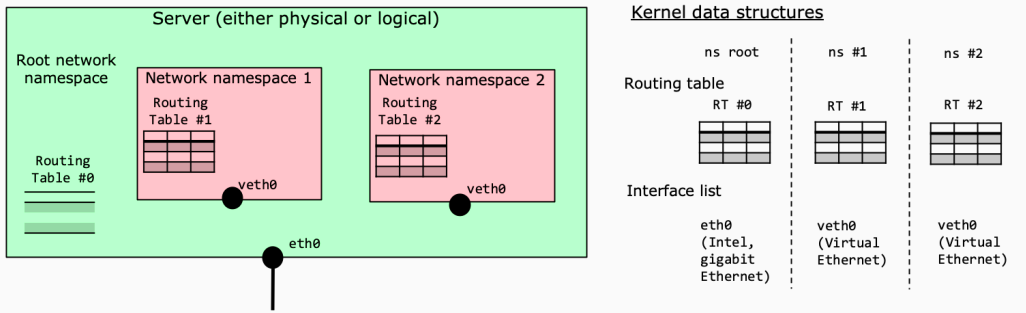
\includegraphics[width=0.6\textwidth, align=c]{namespace-eg.png}}
    \hfill
    \subfloat{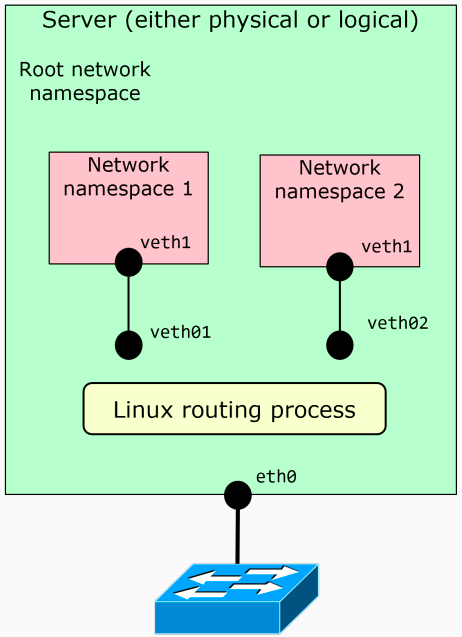
\includegraphics[width=0.3\textwidth, align=c]{namespace-eg2.png}}
    \caption{\emph{Network namespaces} examples}
\end{figure}

\paragraph{Other namespaces in short}
\begin{itemize}
    \item \emph{IPC}: creates private inter-process communication resources for
    isolated processes;
    \item \emph{Mount}: enables the creation of a completely new file system
    with the desired structure (it's similr to chroot);
    \item \emph{UTS}: provides isolation of two system identifiers: hostname and
    NIS domain name;
    \item \emph{User}: allows a process to have root privileges within the
    \emph{namespace} without giving the very same access outside it;
    \item \emph{Cgroups}: provides a mechaism to virtualise the view of the
    \texttt{/proc/\$PID/cgroup} file and \emph{cgroup} mounts;
\end{itemize}

\subsection{Linux containers}
\emph{Linux cgroups} and \emph{namespaces} show some limitations beyond
process isolation. In fact, they provide a way to accomplish virtualization on
a single server, but can't be used on an entire datacenter. Then, they're
flexible, but really hard to use, because they require a lot of commands to
set up a simple isolated environment. Also, they cannot guarantee portability
because there isn't an easy way to package and move them to another server;
hence, when it comes to portability, \emph{VMs} are still preferable. So, \emph{cgroups}
and \emph{namespaces} need to be extended and made easier to use; \emph{Linux
containers} go in this direction.

Containers provide a \emph{lightweigth virtualization} that allows processes and
resources isolation without the complexity of \emph{full virtualization}. They
are an \emph{OS-level virtualization} method for running isolated Linux
systems, called containers, on a single control host and over the same shared
kernel.

\emph{Containers} can group processes together inside an isolated environment,
to which different resources can be assigned and, as we said earlier, they share
the same kernel as the host. From the inside, each \emph{container} looks like
an indipendent machine, while from the outside they're seen as normal processes.

On the other hand, they don't emulate software and can't use a different kernel.
Also, security isn't guaranteed by the model itself, although an appropriate
level of security can still be achieved.

\begin{figure}[ht!]
    \centering
    \subfloat[\emph{Containers architecture}]{
        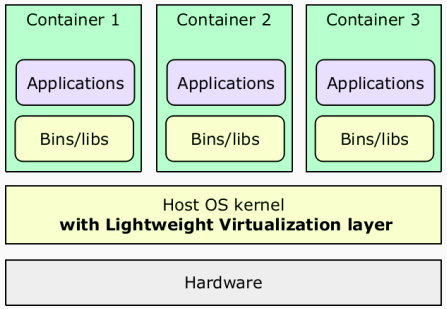
\includegraphics[width=0.3\textwidth]{containers-architecture.png}
    }
    \hspace{2.5cm}
    \subfloat[\emph{Hypervisors architecture}]{
        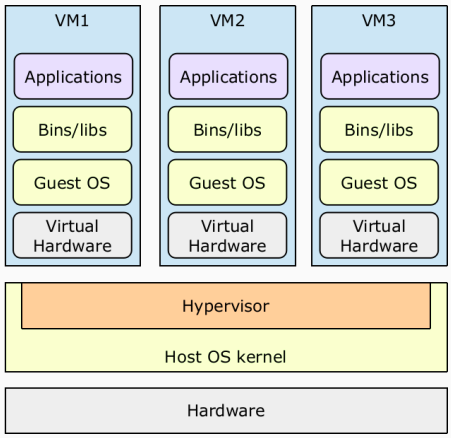
\includegraphics[width=0.3\textwidth]{VMM-architecture.png}
    }
    \caption{\emph{Containers VS Hypervisors architecture}}
\end{figure}

\noindent
Compared to \emph{VMs}, \emph{containers} are both faster and ligher in terms of
resource usage. Hence, a larger number of \emph{containers} can cohexist on
a single host. However, \emph{VMs} still provide better isolation (e.g. kernel
exploits don't affect other \emph{VMs}) and security, as mentioned before.

\begin{note}
    \emph{Linux containers} can both be seen as infrastructure primitives
    (aka \q{lightwieigth \emph{VMs}}) and an application management and
    configuration system.
\end{note}

\paragraph{LXC - Linux Containers in practical}
What we've talked about until now are the general characteristics of
\emph{containers} in a Linux system. \emph{LXCs} (\emph{LinuX Containers}) are
the actual implementation of that technology. They're implemented using
\emph{cgroups}, \emph{namespaces} and other technologies such as Apparmor and
SELinux profiles that allow them to obtain bettere security performance.

So, \emph{LXCs} make it easier to create and manage isolated environments, but
they still lack in resource isolation, because the resource quota of a container
might be affected by others, and both checkpointing and migration, because those features
are not provided by the Linux kernel and third party tools aren't 100\% effective,
yet. Another important limititantion is on portability, because they cannot be
transfered across servers without recreating them.

\subsection{Docker}
So far, we've been able to obtain some form of \emph{lightweigth virtualization},
but we still struggle when it comes to packaging and deployment of environments
and applications in them. \emph{Docker} focuses on applications,
simplifying their deployment and execution by creating a lightweigth, portable
and self-contained \q{package} that runs everywhere.

\emph{Docker} aims to obtain a clean separation of environments, an easy
way to manage resources, applications (e.g. a unified \q{run} command for all
apps) and networking (e.g. Docker bridge, transparent NAT, \dots). Therefore,
\emph{Docker} is not a virtualization engine because it leverages existing
primitives such as \emph{cgroups} and \emph{namespaces}.

Summarizing, we can say that \emph{Docker} is ment to make applications run
consistently in different machines regardless of kernel version, operating
system distribution (it needs to be a Linux distro, tho) and network settings.
Also, it makes separation of concerns easy: developers can focus on what there
is inside the container (e.g. libraries, binaries, \q{manifest}, \dots), devOPs
can focus on the outside (logging, monitoring, remote access, \dots).

\paragraph{Docker VS LXC}
\emph{Docker} is optimized for the deployment of applications, as opposed to
\emph{LXCs} that focus more on containers as lightweigth machines. Then,
\emph{Dockers} containers are portable across machines, while \emph{LXCs} need
to be rebuilt.

\subsection{Docker usage in general}
\emph{Docker} distinguishes between images and containers. The first are
immutable templates for containers that can be pushed and pulled from a registry.
The seconds, on the other hand, are instances of an image that can be started,
stopped, etc. Thus, they maintain their state within their file system.

As mentioned, images can be stored and retrieved from a registry that can
either be public (e.g. Docker hub) or private. Then, given an image, \emph{Docker}
offers a unified interface for creating a container via the \texttt{docker run}
command.

\paragraph{Docker network management}
By default, all containers are connected to a \texttt{docker0} bridge and
\emph{Docker} automatically implements a private IP network with its address
space and the appropriate routing table and iprules for internet connectivity.

\begin{figure}[h!]
    \centering
    \img{docker-network.png}{0.4}
    \caption{\emph{Docker} network setup}
\end{figure}

\noindent
This way, \emph{Docker} provides automatically inbound connection, meaning that
containers running on the same \emph{Docker host} can communicate with each other
without additional configurations. To communicate with the \emph{Docker host}
itself or with other hosts, one or more container ports have to be exposed.

It's interesting to point out that \emph{Docker} doesn't use a DHCP server
to assign IP addresses. Instead, network operations are carried out by a
\texttt{libnetwork} component that implements the \emph{Container Network
Model} (\emph{CNM}). This component decides what IP address to use within the
container, and configures the inside endpoint of the virtual interface to
which that address has been assigned.

\paragraph{Docker file system management}
Since containers must replicate the entire file system required for them to
run, \emph{Docker} must assure that no host  file is accessed from within the
container and that each container holds all that files required to run.
Hence, \emph{Docker} must grant isolation and portability.

\begin{note}
    Whereas containers need to hold all their files, each container might
    weigth hundreds of megabytes.
\end{note}

\noindent
To comply with the requirements above, \emph{Docker} uses a \emph{union file
system}. A \emph{union file system} works on top of other file systems, and
it gives a single, coherent and unified view to file and directories of
separate file systems. In other words, it mounts multiple directories to a
single root, in fact, it is more of a mounting system rather than a file
system. There are different types of union file systems, \emph{Docker} in
particular uses \emph{OverlayFS}.

\begin{figure}[h!]
    \centering
    \img{union-file-system.png}{0.4}
    \caption{Behaviour of a \emph{union file system}}
\end{figure}

\noindent
A \emph{union file system} can be seen as a logical merge of multiple layers in
which only the upper layer is writable; all the lower layers are read only.
When a process wants to read from a file, it starts searching it from the
upper layer, than moves to the lower ones until it isn't found. When accessing
a file in write mode instead, the file system copies that file for that process
(i.e. container) only. All the other processes continue to use the original one.
When it comes to file (or directory) removal, if it resides in the upper layer,
it is removed directly, and it's simulated through a \emph{whiteout} file in
lower layers. This kind of file exists only in \texttt{union} directory, whitout
physically appearing in neither the upper not lower layers.

Such a behaviour of \emph{union file systems} allows multiple containers to
share the same files and directories until they need to modify them. This
reduces the disk fooprint of containers on \emph{Docker host} and their loading
time.

\begin{figure}[h!]
    \centering
    \captionsetup[subfloat]{singlelinecheck=false, width=40mm,
    justification=raggedright}
    \subfloat[Original app]{\hspace{5mm}\img{ufs-1.png}{0.1}}
    \hspace{1.5cm}
    \subfloat[Copy of the app]{\hspace{5mm}\img{ufs-2.png}{0.1}}
    \hspace{1.5cm}
    \subfloat[Modified app]{\hspace{5mm}\img{ufs-3.png}{0.1}}
    \caption{Files sharing into a \emph{union file system}}
\end{figure}

\noindent
\emph{Docker} images are created exploting this behaviour. In fact, any
image results from adding information on top of another image.

\paragraph{Automatic build}
\emph{Docker} allows developers to automatically create a container starting from
its composing elements. The recipe used to create the container is stored in a
file called \texttt{Dockerfile} in which developers can write all the
instructions that have to be executed to set up the container. Using a tool
called \texttt{docker-compose}, multi-container applications can be configured
and deployed using the single command \texttt{docker-compose up}. Finally,
various \emph{Docker host} can be turned into a single virtual host through
\emph{container orchestration tools} such as \emph{Docker swarm} and
\emph{Kubernetes}.